% Chapter 1

\chapter{Memory Complexity} % Main chapter title

\label{Chapter6} % For referencing the chapter elsewhere, use \ref{Chapter1} 

%----------------------------------------------------------------------------------------

% Define some commands to keep the formatting separated from the content 
%\newcommand{\keyword}[1]{\textbf{#1}}
%\newcommand{\tabhead}[1]{\textbf{#1}}
%\newcommand{\code}[1]{\texttt{#1}}
%\newcommand{\file}[1]{\texttt{\bfseries#1}}
%\newcommand{\option}[1]{\texttt{\itshape#1}}

%----------------------------------------------------------------------------------------


In this section we provide a method for applying dimensional reduction of the multidimensional scenario, by grouping significant small subsets of the data and concatenating them after embedding. 


\section{Definition}

We define a generalized ID function by:

\begin{equation}
ID_(\overrightarrow{x_1} , \overrightarrow{x_2} ; S) = [ ID(\overrightarrow{x_1}_[S_1],\overrightarrow{x_2}_[S_1]) , \dots , \dots , ID(\overrightarrow{x_1}_[S_g],\overrightarrow{x_2}_[S_g])  ]
\end{equation}

where $S$ is the defined sub-domain group: \\ 

$\{S_i\}_{i=1}^g \qquad,\qquad S_i\subseteq [1, \dots , n] \qquad , \qquad g \in [1, \dots , n]$ \\ 

Where $g$ represents a sub domain which extracts valid demandable information to the user. \\ \\ \\


For example when applying ID embedding on \textbf{SIFT[]} descriptors, a certain user may involve only neighbor pairs, where another one may involve just bin-to-bin pairs.

\subsection{SIFT Example}

when applying ID on SIFT [] descriptors (for template matching),  n is 128, which causes time and memory complexity to be scaled by 1282=16384. 
If one user desires, and physically ables to reduce this coefficient, we developed the following generalization.

\begin{figure} \label{s1}
	    \centering
		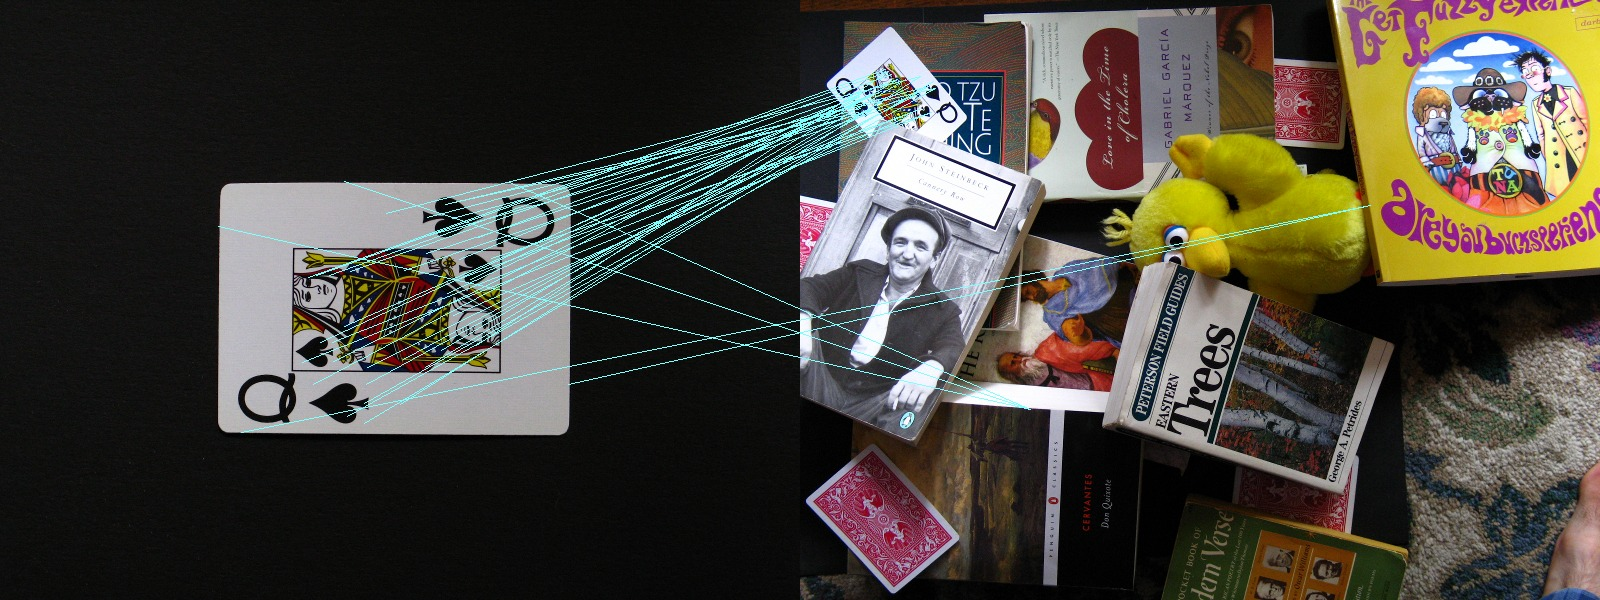
\includegraphics[width=\linewidth,height=12cm,keepaspectratio]{Figures/sift1}
		\caption[flattening 2d matrix]
		{flattening 2d matrix to row-wise 1d vector}
	
\end{figure}
	
	
	
\begin{figure} \label{s2}
		\centering
	
		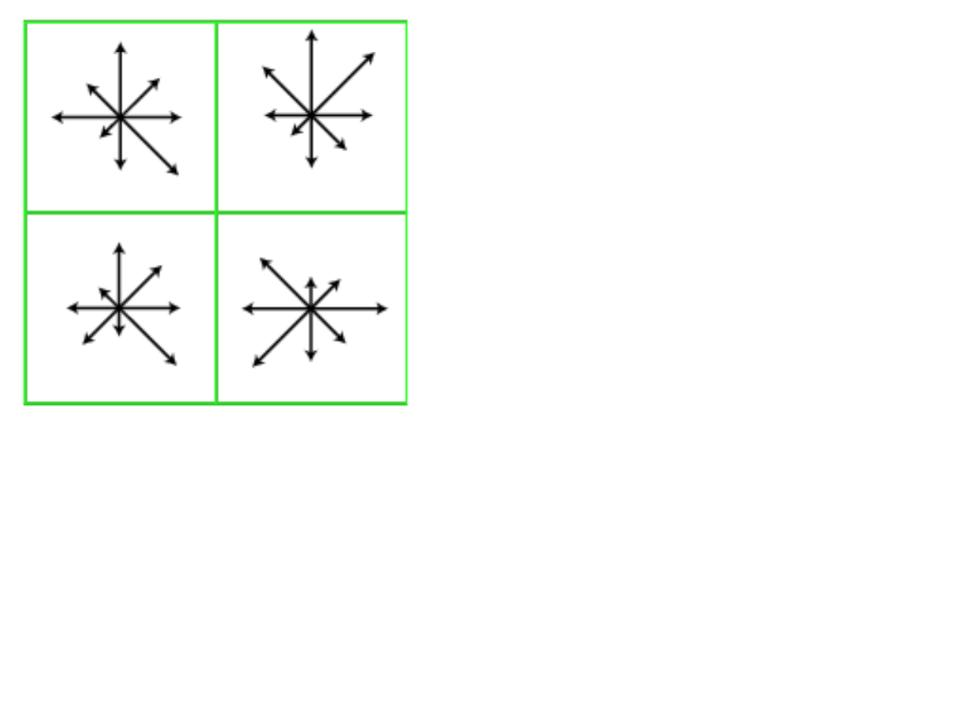
\includegraphics[width=12cm,height=12cm,keepaspectratio]{Figures/sift2}
		\caption[flattening 2d matrix]
		{flattening 2d matrix to row-wise 1d vector}
	
\end{figure}

